
\documentclass{beamer}

\input ./packages.tex
\input ./macros.tex

\usepackage{tikz}

\title{\textcolor{LegoBlueprintBlack}{\textbf{How to build great transport in ex-soviet cities!} - for dummies}}
\author{Jozef Labuš}
\date{2024}

\begin{document}
\begin{frame}[plain, label=current]
\transfade
\begin{tikzpicture}[remember picture,overlay]
    \node[at=(current page.center)] {
	\only<1>{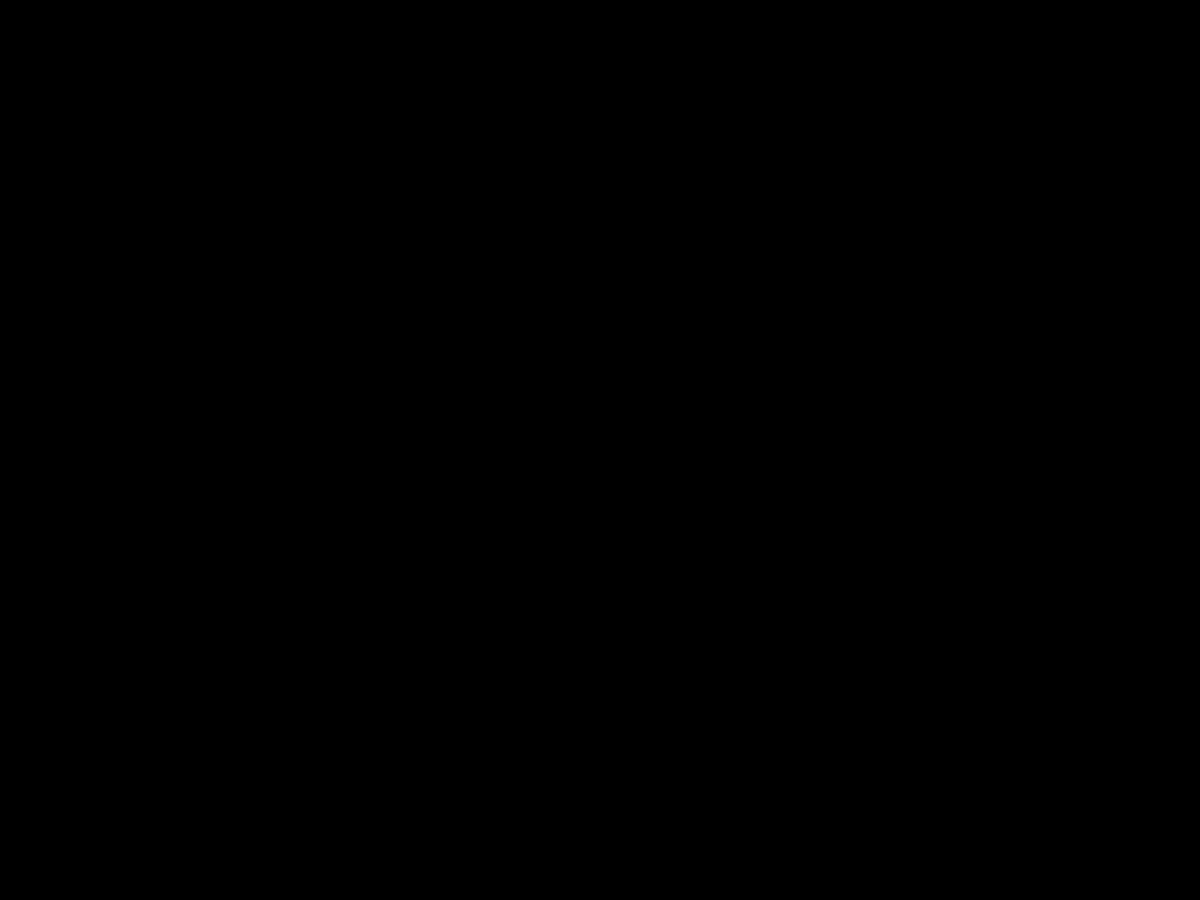
\includegraphics[width=1.01\paperwidth]{black}}
	\only<2>{
\includegraphics[width=1.01\paperwidth]{matrix}}
    };
\end{tikzpicture}
\end{frame}

\begin{frame}[plain]
	\begin{columns}
		\begin{column}{0.5\textwidth}
			\includegraphics[width=\textwidth]{intro}
		\end{column}
		\begin{column}{0.5\textwidth}
			\titlepage
		\end{column}
	\end{columns}
\end{frame}

\begin{frame}
	\begin{enumerate}
		\item Prologue - history of transport in Bratislava + theory
		\item Present - evaluating the present transport in Bratislava today and what should be done about it
		\item Future - problems we are gonna face

	\end{enumerate}
\end{frame}

\input ./sections/prologue.tex
\input ./sections/present.tex
\input ./sections/future.tex
\end{document}
